\documentclass{beamer}
\usepackage{tikz}
\usepackage{xcolor}
\usetheme{Copenhagen}
%Information to be included in the title page:
\title{\bfseries What factors predict S\&P500?}
\author{J. Cavegn, A. Falk, J. Raschke}
\institute{UZH, Department of Banking and Finance}
\date{2023}



\logo{
\includegraphics[height=1cm]{images/UZH_logo.png}}
\begin{document}

\frame{\titlepage}

\begin{frame}
\frametitle{Table of Content}
\tableofcontents
\end{frame}

\begin{frame}
\frametitle{Introduction}
\begin{itemize}
\item Prediction of S\&P 500 returns with an emphasis on currency data
\item Examine whether fluctuations in exchange rates can serve as a real-time signal for future S\&P 500 returns
\item Three supervise machine learning models used to capture possible complex interplay between FX rates and the equity markets:
\begin{itemize}
\item Support Vector Machine
\item Decision Tree Classifier 
\item Random Forest Classifier
\end{itemize}
\item Detailed information about the implementation (functions and code) can be found in the full report
\end{itemize}
\end{frame}

\begin{frame}
\frametitle{Support Vector Machine}
\begin{itemize}
\item Supervised machine learning model for classification and regression tasks
\item Idea: Find the hyperplane that best separates the data into distinct classes while maximizing the margin between them
\item SVM's ability to handle high-dimensional data and capture non-linear relationships makes it a valuable tool for investigating the intricate relationships between FX rates and equity markets
\end{itemize}
\end{frame}

\begin{frame}
\frametitle{Decision Tree Classifier}
\begin{itemize}
\item Decision trees are hierarchical tree-like structures that recursively split the dataset based on feature conditions
\item Idea: Splits are determined by selecting the features that maximize information gain or minimize impurity at each node
\item Decision trees are intuitive models that can capture complex decision boundaries and are easily interpretable markets
\item Parameters: Maximum depth, which controls the complexity of the model 
\end{itemize}
\end{frame}

\begin{frame}
\frametitle{Random Forest Classifier}
\begin{itemize}
\item Random Forest Classifier combines several decision trees and combines their predictions
\item Idea:  Each tree is trained on a random subset of the data, and the final prediction is obtained through a voting mechanism
\item  Random Forest enhances model robustness and generalization by mitigating overfitting. By aggregating the outputs of individual trees, we aim to improve the overall accuracy and reliability of our predictive model.
\item Parameters: 
    \begin{itemize}
    \item Trees: Number of decision trees in the "forest" 
    \item Maximum depth: The maximum depth of one decision tree in the forest
    \item Leaves: Number of terminal nodes in one tree
    \end{itemize}
\end{itemize}
\end{frame}

\begin{frame}
\frametitle{Initial Results}
\begin{itemize}
\item The idea of all three models is to predict an up or down-move of the S\&P 500, in which case they can take a long or short position to profit from the anticipated move (in the code, there is a setting for allowing short positions)
\item Initially, the three models were trained with all available currencies as predictor variables, a lag of one day, 0.8 training/test set split, allowing both long and short positions. All other parameters were set to their default values as specified in the report.
\item Prediction accuracies are displayed in the table below:
\end{itemize}
\begin{table}[h]
  \centering
  \begin{tabular}{lcc}
    \hline
    Classifiers & In Sample & Out-of-Sample \\
    \hline
    SVC & 0.581024 & 0.510906 \\
    DTC & 0.624265 & 0.477349 \\
    RFC & 0.564442 & 0.510067 \\
    \hline
  \end{tabular}
  \caption{Performance of Classifiers}
  \label{tab: classifier_performance}
\end{table}
\end{frame}

\begin{frame}
\frametitle{Initial Results}
\begin{itemize}
\item As can be gathered from the table in the previous slide, out of sample performance is not better than flipping a coin. \item Additionally, as seen in figure \ref{fig: cumulative returns} (GIF) below, RFC and DTC backtesting performances are heavily seed-dependent
\end{itemize}
\begin{figure}[h!]
\begin{center}
  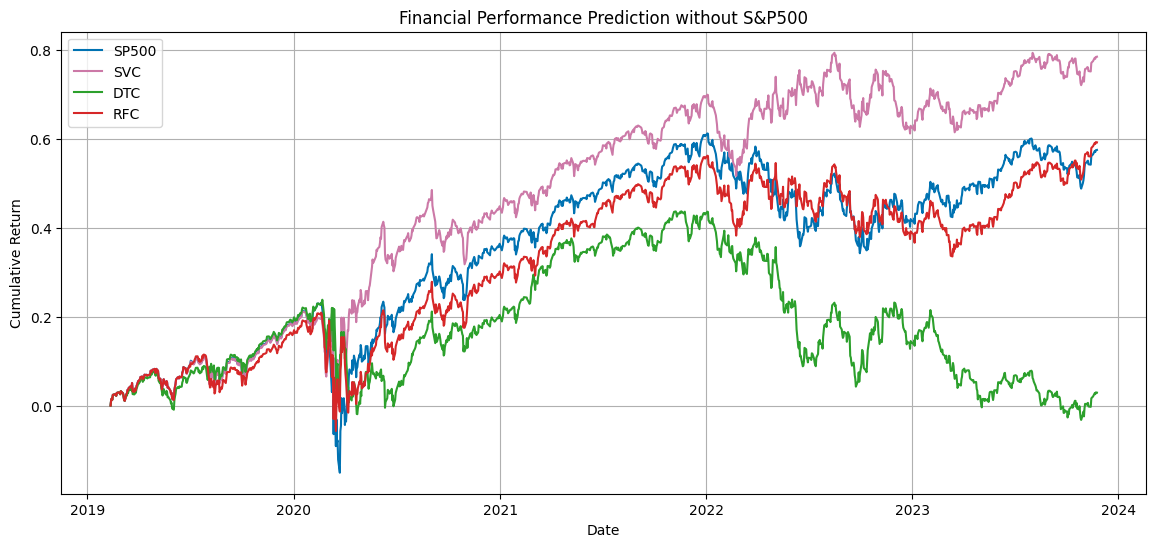
\includegraphics[width=0.7\columnwidth]{images/first_visualization.png}
  \caption[Model return comparison]{Cumulative returns of all three models compared to the long only S\&P500.}
  \end{center}
  \label{fig: cumulative returns}
\end{figure}
\end{frame}

\begin{frame}
\frametitle{Simulation}
\end{frame}

\begin{frame}
\frametitle{Finding the best predictor (SVM)}
\begin{itemize}
    \item Here we analyze the best currency combinations (as predictor variables) ranked by backtesting performance for the SVM model
    \item With 10 different currencies, there are 1023 combinations of currencies. The highest performing combination with a return of 114\% is EUR, JPY, CAD, SEK and SGD
    \item The reason for the high returns is due to being short the S\&P 500 during the 2020 COVID-19 stock market crash
    
\end{itemize}
\end{frame}

\begin{frame}
\frametitle{Finding the best predictor (SVM)}
\begin{itemize}
    \item The following plot shows the 1023 predictor variable combinations with the aforementioned best one marked in blue:
\end{itemize}
\begin{figure}[h!]
\begin{center}
  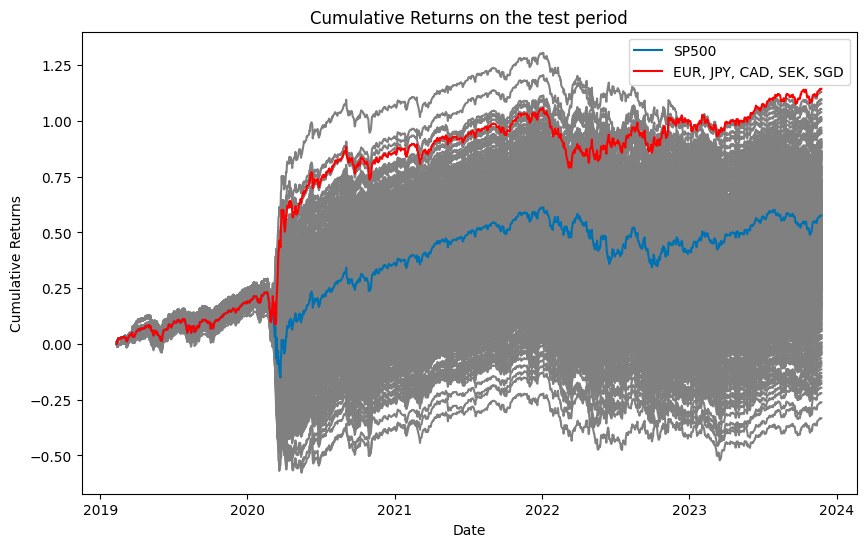
\includegraphics[width=0.6\columnwidth]{images/best_predictor.png}
  \caption{Cumulative returns of all different currency combinations used as explanatory variables.}
\end{center}
  \label{fig: cumulative returns}
\end{figure}
\end{frame}

\begin{frame}
\frametitle{Finding the best predictor (SVM)}
\begin{itemize}
    \item The figure below shows the distribution of the cumulative returns of backtests of all currency combinations:
\end{itemize}
\begin{figure}[h!]
\begin{center}
  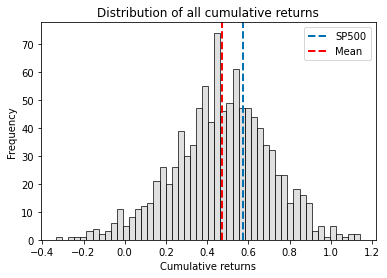
\includegraphics[width=0.55\columnwidth]{images/hist_comparison.png}
  \caption{Cumulative returns of all different currency combinations used as explanatory variables.}
\end{center}
  \label{fig: cumulative returns}
\end{figure}

\end{frame}


\begin{frame}
\frametitle{Finding the best predictor (SVM)}
 \begin{itemize}
     \item slides for simulation stuff
     \item appendix slide about playground (also add to report)
     \item align color scheme
     \item double check the decimal package thing...
     \item add mention of memoization to report somewhere
     \item make table of contents, bibliography
 \end{itemize}
\end{frame}


    


\end{document}
